
\documentclass[superscriptaddress, twocolumn, prd]{revtex4-1}
\usepackage[latin9]{inputenc}
\usepackage{amsmath}
\setcounter{secnumdepth}{3}
\usepackage{amstext}
\usepackage{graphicx}
\usepackage{physics}
\usepackage{changes}

\begin{document}

\title{A Pseudo Plane-wave Gravitational Calibrator for Gravitational Wave Observatories}

\author{M.P. Ross}
\email[]{mpross2@uw.edu}
\author{E.G. Adelberger}
\author{C. Weller}
\author{J.H. Gundlach}
\affiliation{Center for Experimental Nuclear Physics and Astrophysics, University of Washington, Seattle, Washington,
98195, USA}
\author{Timesh Mistry}
\affiliation{The University of Sheffield, Sheffield S10 2TN, UK}
\author{Laurence Datrier}
\affiliation{SUPA, University of Glasgow, Glasgow G12 8QQ, UK}
\author{Jeff Kissel}
\affiliation{LIGO Hanford Observatory, Richland, WA 99352, USA}


\begin{abstract}

Gravitational calibration has recently gained interest as a possible improvement to gravitational wave observatories. Many gravitational calibrators are limited by their dependence on the relative position between the calibrators and the test masses. Here we present a novel geometry consisting on eight quadrupole rotors placed at the vertices of a cube centered on the test mass. The phases and rotation directions are selected to produce a pseudo plane-wave  sinusoidal gravitational acceleration with amplitude of \added{$368.46$ fm/s$^2$}. This acceleration has minimal positioning dependence and can yield \added{$\sim0.1 \%$} acceleration amplitude uncertainty for \added{$\sim$1 cm} test mass positioning uncertainty. In addition, these rotors have significant engineering and safety benefits due to their small size and eliminates the torques acting on the test mass.

\end{abstract}

\maketitle

\section{Introduction}

Gravitational wave astronomy has blossomed into a novel method to observe the universe. The number of gravitational wave observations is expected to grow substantially in the coming years with the continued operation of the LIGO \cite{aLIGO} and Virgo \cite{virgo} interferometers as well the future addition of LIGO-India \cite{ligo-india} and the further improvements of KAGRA \cite{kagra}. 

These interferometers must be precisely calibrated in order to accurately interpret gravitational wave signals. Whether for binary merger parameter estimation \cite{abbott2020population}, cosmological measurements \cite{abbott2021gravitational, ligo2017gravitational}, or searches for deviations from general relativity \cite{abbott2020tests}, the strain readouts of the observatories must be precisely and accurately calibrated.

Thus far, the calibration of the current observatories has been accomplished with photon pressure \cite{PCal}. These photon calibration systems have yielded absolute calibrations with \added{$\sim0.5\%$} uncertainty and have acted as versatile calibration tools. 

Calibrating with a gravitationally induced strain has long been suggested as an alternative calibration technique \cite{hirakawa1980dynamical, kuroda1985experimental, mio1987experimental, astone1991evaluation, astone1998experimental, Matone_2007} and has recently been explored at many of the observatories \cite{Estevez_2018, estevez2021newtonian, PhysRevD.98.022005, ncal}. Gravitational calibration has the promise of improving the absolute calibration of the observatories by achieving higher-precision injections. Additionally, gravitational calibrator can work in concert with photon calibrator to yield a lower uncertainty combined calibration.

The geometries explored with current gravitational calibrators \cite{Estevez_2018, estevez2021newtonian, PhysRevD.98.022005, ncal} produce accelerations that have large dependence on the radial distance, $r$, between the rotor and the test mass. The acceleration is typically proportional to $\sim1/r^{l+2}$ where $l$ is the order of the dominate mass-multipole moment. For example, a rotor with a quadrupole mass distribution ($l=2$) will follow $\sim1/r^4$. This strong positioning dependence causes the performance of the absolute calibration to be limited by the precision of the positioning measurements. 

Here, we present a novel geometry consisting of eight quadrupole rotors that produces a pseudo plane-wave gravitational acceleration. This geometry produces an acceleration which has minimal first-order dependence on the position of the rotors allowing for improved calibration precision with limited positioning precision. Additionally, this geometry eliminates the torques acting on the test mass and eases much of the engineering and safety concerns of previous rotors.

\begin{figure}[!h]
\centering 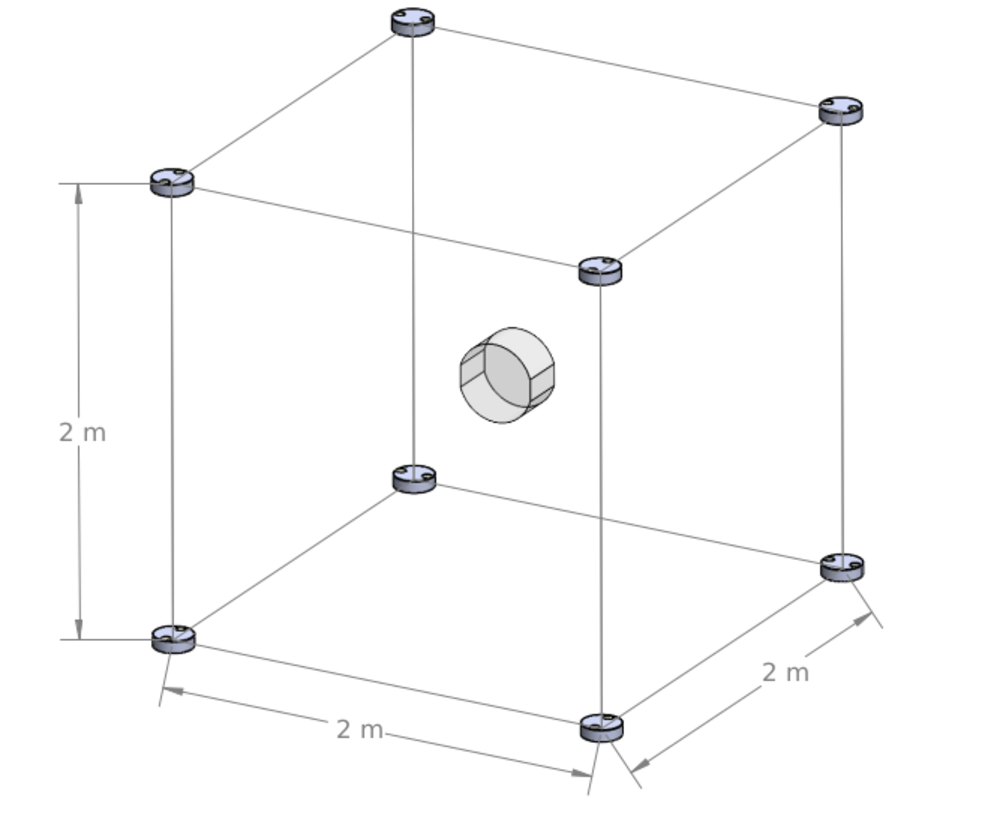
\includegraphics[width=0.5\textwidth]{Super8_Model.pdf}
\caption{A rendering of the geometry of the rotors with the test mass at the center of the cube.}
\label{cad} 
\end{figure}

\section{Geometry}

The pseudo plane-wave calibrator consists of eight identical rotors placed at the vertices of a $2$ meter sided cube centered on the test mass. Figure \ref{cad} shows a rendering of the geometry. The rotors are designed with the similar dimensions as the LIGO NCal \cite{ncal} but without a hexapole mass arrangement. Each rotor is a 17 cm diameter, 5 cm tall aluminum disk with two holes cut at a radius of 6 cm separated by $90^\circ$. These holes are filled in with 4 cm diameter, 5 cm tall  tungsten cylinders which produce a quadrupole mass distribution. The parameters of the geometry are displayed in Table~\ref{param}.

The relative phases of the rotors and the rotation directions are set to achieve pseudo plane-wave nature. The four rotor with a positive x-coordinate are rotated by $90^\circ$ from the rotors with negative x-coordinate. Additionally, the rotors with positive y-coordinate rotate clockwise while those with negative y-coordinates rotate counter-clockwise. 

\begin{widetext}
\begingroup
\setlength{\tabcolsep}{10pt} % Default value: 6pt
\renewcommand{\arraystretch}{1.5} % Default value: 1

\begin{table}[h!]
\begin{center}
\begin{tabular}{ |l|c|c| }
\hline
 Parameter & Mean & Uncertainty \\
 \hline
Cylinder Mass $m$ & 1~kg & 0.3~g \\
Cylinder Radius $r_c$& 2~cm & 2.5 $\mu$m \\
Cylinder Length $l_c$& 5~cm & 5 $\mu$m \\
Quadrupole Radius $r_{q}$ & 6~cm & 5 $\mu$m \\
Test Mass $M$ & 40~kg & 10~g \\
Test Mass Length $l_{tm}$& 200~mm & 0.1~mm\\
Test Mass Radius $r_{tm}$& 170~mm & 0.05~mm\\
Test Mass Flat Width $w_{tm}$& 327~mm & 0.05~mm\\
Rotor Positions $\vec{r}$& ($\pm$ 1 m, $\pm$ 1 m, $\pm$ 1 m) & (1 mm, 1 mm, 1 mm) \\
Test Mass Position $\vec{r}_{tm}$& (0 m, 0 m, 0 m) & (1 cm, 1 cm, 1 cm) \\
 \hline

 \end{tabular}
 \caption{Parameters describing the rotors, the test mass, and their respective positions.}\label{param}
 \end{center}

\end{table}
\endgroup
\end{widetext}

\section{Pseudo Plane-wave Nature}

To verify the performance of such a rotor array, we simulated the system with a finite-element analysis using the \textit{PointGravity} algorithms of the \texttt{newt} libraries \cite{Hagedorn, pgURL}. This simulation breaks each of the rotor cylinders and the test mass into independent clouds of point masses. The force between each pair of point masses, one from the rotors and the other from the test mass, is calculated. The forces from the individual pairs of point masses is then summed to yield the acceleration in all three directions. We extract only the x-acceleration as this is the primary sensitive direction of the interferometer.

The superposition of the gravitational fields from the eight rotors produces an oscillating gravitational acceleration field which at the center of the cube is only in the x-direction and an amplitude of \added{$368.46$ fm/s$^2$}. The acceleration field changes weakly with deviations from the center of the cube (i.e. a pseudo plane-wave). The percentage change in acceleration amplitude verse offset from the center of the cube is shown in Figure \ref{offset} for offsets in each direction. A relatively large offset of 10 cm in any direction changes the acceleration by $<2\%$. Additionally, the change in amplitude is well-described by a parabola for small offsets which displays the second-order nature of this effect. 


\begin{figure}[!h]
\centering 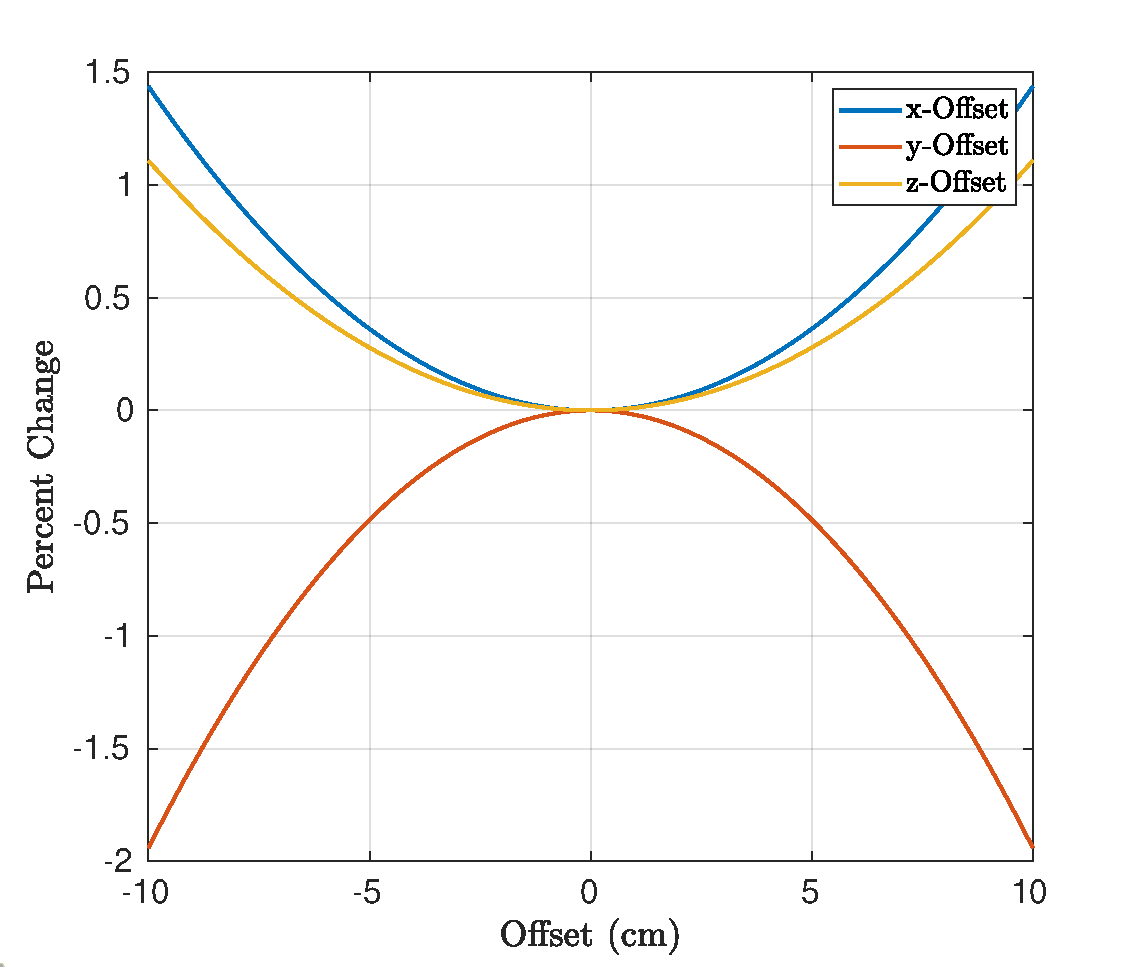
\includegraphics[width=0.5\textwidth]{Super8_PerVsZ.pdf}
\caption{The percentage change of acceleration amplitude with a test mass offset from the center of the cube.}
\label{offset} 
\end{figure}

Since the acceleration is primarily in the x-direction over the volume of the test mass, the rotors apply torques with negligible amplitudes.

\section{Numerical Uncertainty Analysis}

Since the performance of such a calibrator does not only depend on the test mass offset, we performed a Monte Carlo simulation of the applied acceleration to accounting for all of the parameters which describe the calibrator. We model each parameter as a Gaussian distribution centered on the mean listed in Table \ref{param} with $\sigma$-value equal to the uncertainty. The acceleration of the test mass is then calculated with parameters sampled from these distributions. This is repeated \added{2000} times to yield a distribution of the gravitational acceleration, shown in Figure \ref{dist}, which takes into account all non-linearities and degeneracies. 

The simulation yields an injected acceleration of a~=~368.46~$\pm$~0.45 fm/s$^2$~(0.12~\% ) where the central value is the mean and the uncertainty is the 68\%-interval. To assess how each parameter contributes to this total uncertainty, the acceleration uncertainty was recomputed with only one parameter varying. This was then repeated for each parameter to yield the results in Table \ref{uncert}. All eight rotor positions were simultaneously varied  in all three directions and the test mass position was also varied in all three directions.

\begin{figure}[!h]
\centering 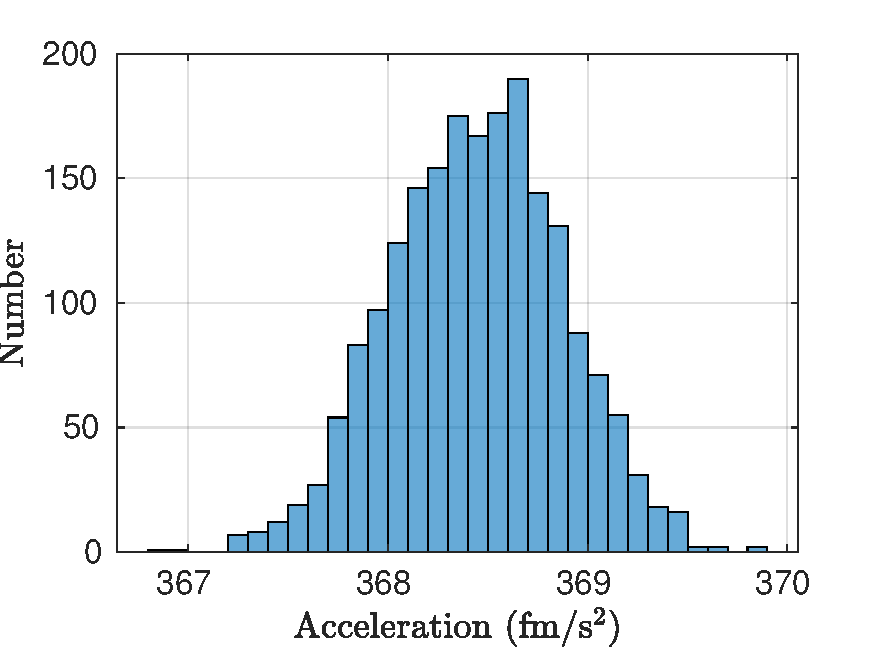
\includegraphics[width=0.5\textwidth]{Super8_Dist.pdf}
\caption{Distribution of predicted accelerations.}
\label{dist} 
\end{figure}


Table \ref{uncert} shows the acceleration uncertainty is strongly dominated by the rotor positions with the test mass position contribution being 3.5 times smaller. Since the rotors would be outside the interferometer's vacuum system, their positions can be readily measured to the mm precision simulated here. This contribution may be further reduced with a precision machined mounting frame for the rotors. 

\begin{widetext}
\begingroup
\setlength{\tabcolsep}{10pt} % Default value: 6pt
\renewcommand{\arraystretch}{1.5} % Default value: 1

\begin{table}[h!]
\begin{center}
\begin{tabular}{ |l|c|c|c| }
\hline
 Parameter & Mean & Uncertainty & Percentage Contribution\\
 \hline
Cylinder Mass $m$ & 1~kg & 0.3~g & $3.68\times10^{-2}$\\
Cylinder Radius $r_c$& 2~cm & 2.5 $\mu$m & $2.91\times10^{-6}$\\
Cylinder Length $l_c$& 5~cm & 5 $\mu$m & $4.28\times10^{-6}$\\
Quadrupole Radius $r_{q}$ & 6~cm & 5 $\mu$m &$1.68\times10^{-2}$\\
Test Mass $M$ & 40~kg & 10~g & $2.61\times10^{-2}$\\
Test Mass Length $l_{tm}$& 200~mm & 0.1~mm& $3.86\times10^{-4}$\\
Test Mass Radius $r_{tm}$& 170~mm & 0.05~mm& $4.90\times10^{-4}$\\
Test Mass Flat Width $w_{tm}$& 327~mm & 0.05~mm&$1.64\times10^{-13}$\\
Rotor Positions $\vec{r}$& ($\pm$ 1 m, $\pm$ 1 m, $\pm$ 1 m) & (1 mm, 1 mm, 1 mm) &$1.22\times10^{-1}$\\
Test Mass Position $\vec{r}_{tm}$& (0 m, 0 m, 0 m) & (1 cm, 1 cm, 1 cm) &$3.46\times10^{-2}$\\
 \hline

 \end{tabular}
 \caption{Individual uncertainty contributions for the input parameters of the simulation.}\label{uncert}
 \end{center}

\end{table}
\endgroup
\end{widetext}

\section{Conclusion}
 
\quad We have described an eight-rotor gravitational calibrator that causes a psuedo-plane wave acceleration field. Simulation of the acceleration amplitude uncertainty show that it can achieve $\sim0.1\%$ precision absolute calibration injections. This is approximately an order of magnitude improvement over previously deployed geometries. 

Although not shown in detail here, similar performance can be achieved with an in-plane, four-rotor system albeit without the minimal z-offset dependence. Such a four-rotor array would cost less to build and may be easier to install around existing equipment.

Gravitational calibration is a promising avenue for high precision absolute calibration of gravitational wave observatories. By deploying arrays which minimize the slope of the applied gravitational field around the test mass, such calibrators may exceed the performance of excising calibration techniques.

\begin{acknowledgements}

Participation from the University of Washington, Seattle, was supported by funding from the NSF under Awards PHY-1607385, PHY-1607391, PHY-1912380, and PHY-1912514.


\end{acknowledgements}


 \bibliographystyle{unsrtnat}
\bibliography{Super8.bib}

\end{document}
